\section{Chasis}
Para facilitar la fabricación se opto por un chasis impreso en 3D para la POC.

Durante el proceso de diseño se tuvieron en cuenta las particularidades del proceso de impresión y los limites de volumen de las impresoras disponibles.

Con el objetivo de utilizar solo dos motores y mantener el movimiento solidario de las ruedas por lado se opto por unir los ejes delantero y trasero de cada lado con cadenas.

El diseño del chasis del robot se puede subdividir en secciones básicas que se unen entre si:

\begin{itemize}
    \item \textbf{Ejes:} Soportan el peso del robot y transmiten la energía a las ruedas.

    \item \textbf{Largueros del chasis:} Proporcionan rigidez y junto con los ejes forman las unidades básicas de tracción del robot.

    \item \textbf{Pisos:} Terminan de conformar la base y proporcionan el lugar para almacenar baterías y la electrónica.

    \item \textbf{Coraza superior:} Da soporte a los componentes externos y la torreta. 

    \item \textbf{Torreta:} Da soporte y permite apuntar el arma, telémetro y la cámara principal. 

\end{itemize}

\subsection{Análisis de Implementación}

A continuación, se presenta un análisis detallado de las secciones básicas del chasis del robot y su implementación


\subsubsection{Ejes}

Los ejes tienen que soportar el peso del robot y al mismo tiempo transmitir la rotacion de los motores a las ruedas traseras y delanteras de cada lado de manera solidaria. Por esta razon se decidieron usar dos rulemanes de apoyo para soportar el peso de manera mas estable y se decidio agregar un piñon para unir las ruedas delanteras y traseras de cada lado con una cadena.

La estructura se compone de un eje central de metal, con los alojamientos para los dos rulemanes de apoyo, el piñón y el plato que sostiene la llanta, el cual tiene una chaveta para evitar que gire.

Los motores de tracción se fijan a los ejes con prisioneros que traban en el biselado de los ejes de los motores.

\begin{figure}[H]
\centering
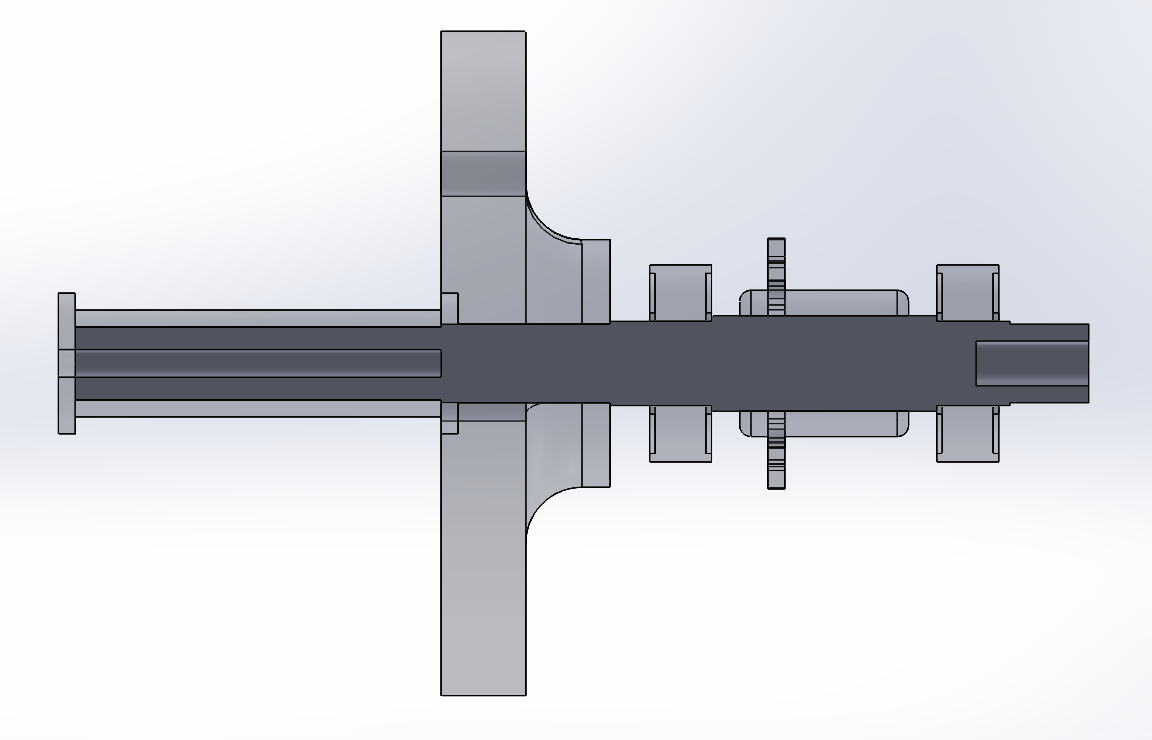
\includegraphics[width=1\textwidth]{Figures/eje_corte.png}
\label{fig:eje}
\caption{Corte del eje}
\end{figure}

\subsubsection{Largueros del chasis}

Los encargados de dar soporte a los ejes y mantener las cadenas de transmisión en su lugar son los largueros del chasis, los cuales son las piezas centrales en la estructura de la plataforma y junto con los motores y ruedas forman las unidades básicas de tracción del robot.

Se componen de 7 secciones, de las cuales 6 son la estructura del larguero y una ultima el soporte para el motor de tracción. En caso de cambiar a un esquema de 4 motores de tracción solamente es necesario agregar una placa de soporte extra delante ya que el diseño es simétrico.

Estas piezas deben ser ensambladas alrededor de los ejes de tracción ya que también limitan el movimiento axial de los rulemanes.

\begin{figure}[H]
\centering
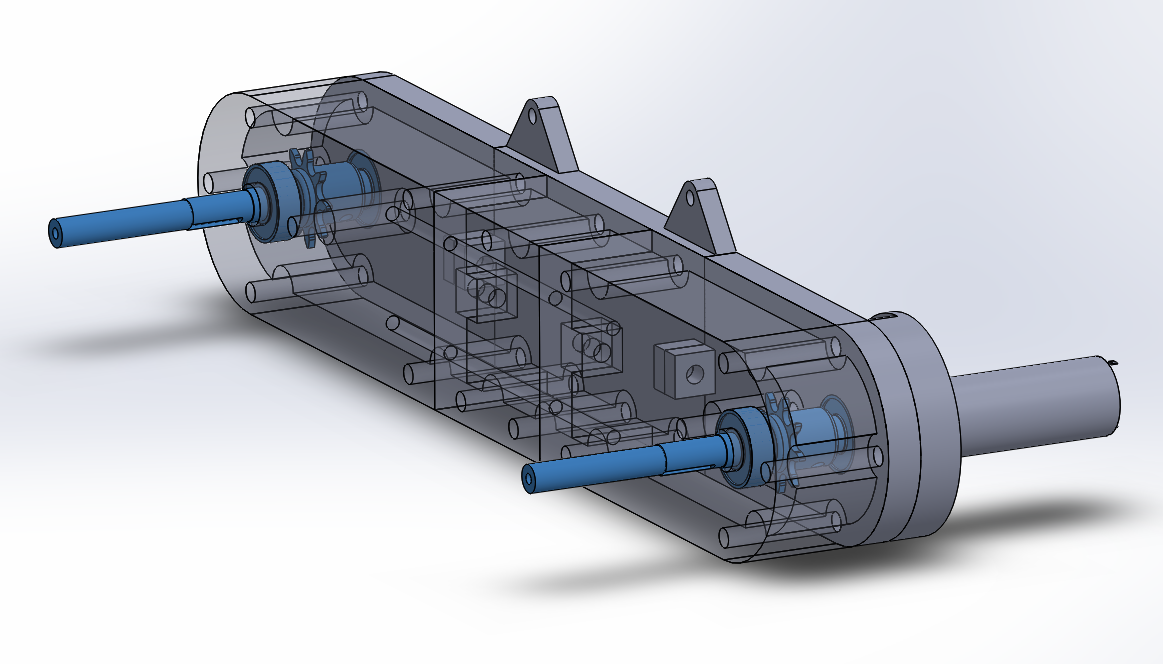
\includegraphics[width=1\textwidth]{Figures/larguero.png}
\label{fig:base}
\caption{Largueros del chasis}
\end{figure}

\subsubsection{Pisos}

Los pisos se agregan a los largueros para terminar de conformar la estructura de la plataforma, la cual esta diseñada por secciones imprimibles que luego se unen entre si con varillas transversales para dar rigidez y fuerza al conjunto.

\begin{figure}[H]
\centering
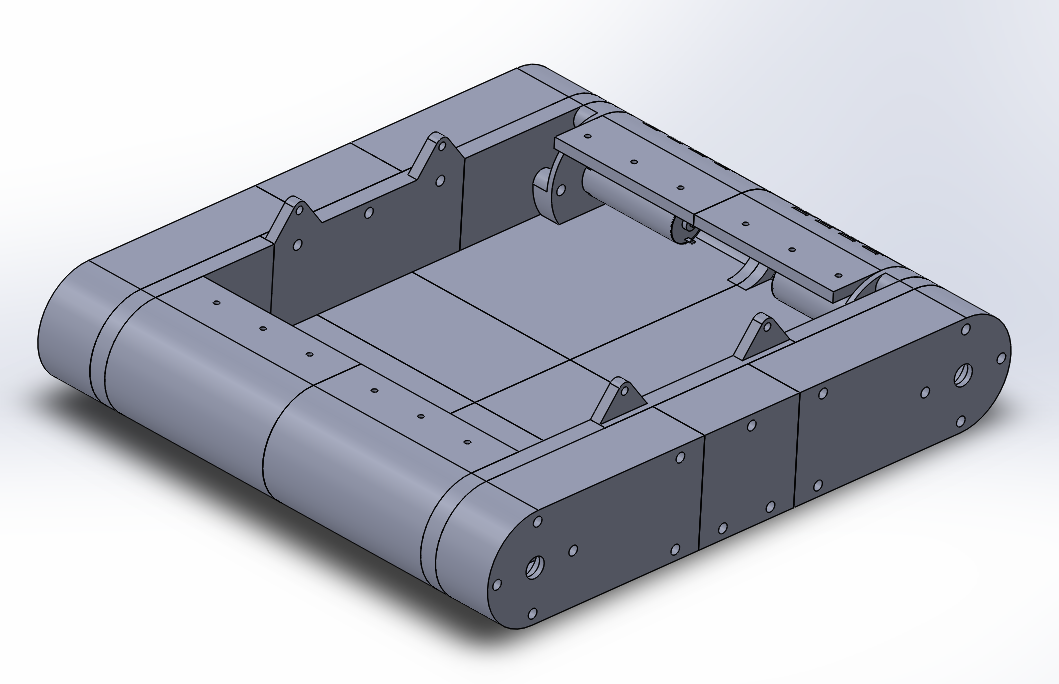
\includegraphics[width=1\textwidth]{Figures/base_sola.png}
\label{fig:base}
\caption{Base del robot}
\end{figure}

\subsubsection{Coraza superior}

La coraza superior se diseño con forma de caparazón angulado, con una apertura para el sensor LIDAR y una plataforma para llevar la PC (que para simplificar las pruebas se dejo afuera del prototipo).

En el diseño de la coraza también se busco solucionar la limitación en el volumen de impresión por lo que se diseño una estructura con piezas que se intercalan para obtener rigidez, lo cual es esencial ya que la coraza da soporte a la torreta principal.

\begin{figure}[H]
\centering
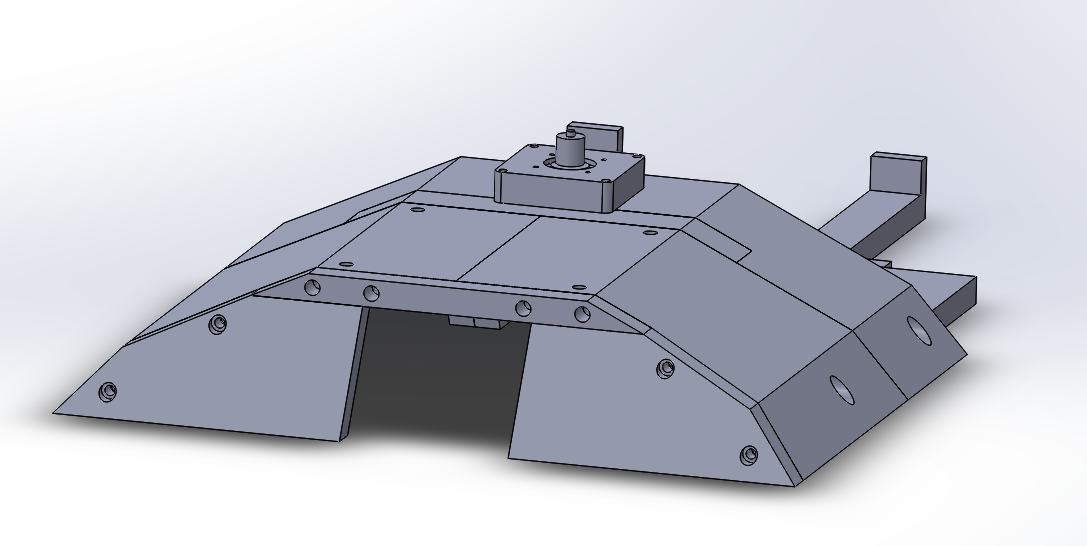
\includegraphics[width=1\textwidth]{Figures/coraza sola.png}
\label{fig:base}
\caption{Coraza superior}
\end{figure}

\subsubsection{Torreta}

La torreta se compone de una plataforma giratoria para el eje X que se conecta al motor con una correa y sobre esta plataforma se monto el soporte del motor y el arma con la articulación del eje Y.

El arma se agarra de un aplique fijo en su riel, en posición invertida.

\begin{figure}[H]
\centering
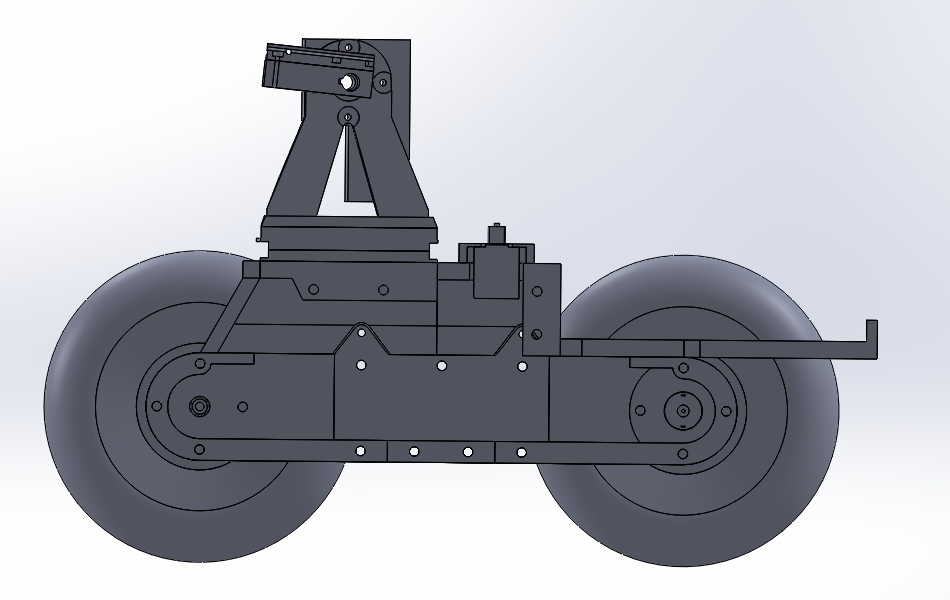
\includegraphics[width=1\textwidth]{Figures/corte robot.png}
\label{fig:robot}
\caption{Corte lateral del robot}
\end{figure}

\subsubsection{Ensamblaje completo}

Las partes superior e inferior de la coraza se ensamblan con 4 encastres triangulares, lo cuales adicionalmente se aseguran con 4 tornillos y se conforma entonces la estructura completa del chasis del prototipo.

\begin{figure}[H]
\centering
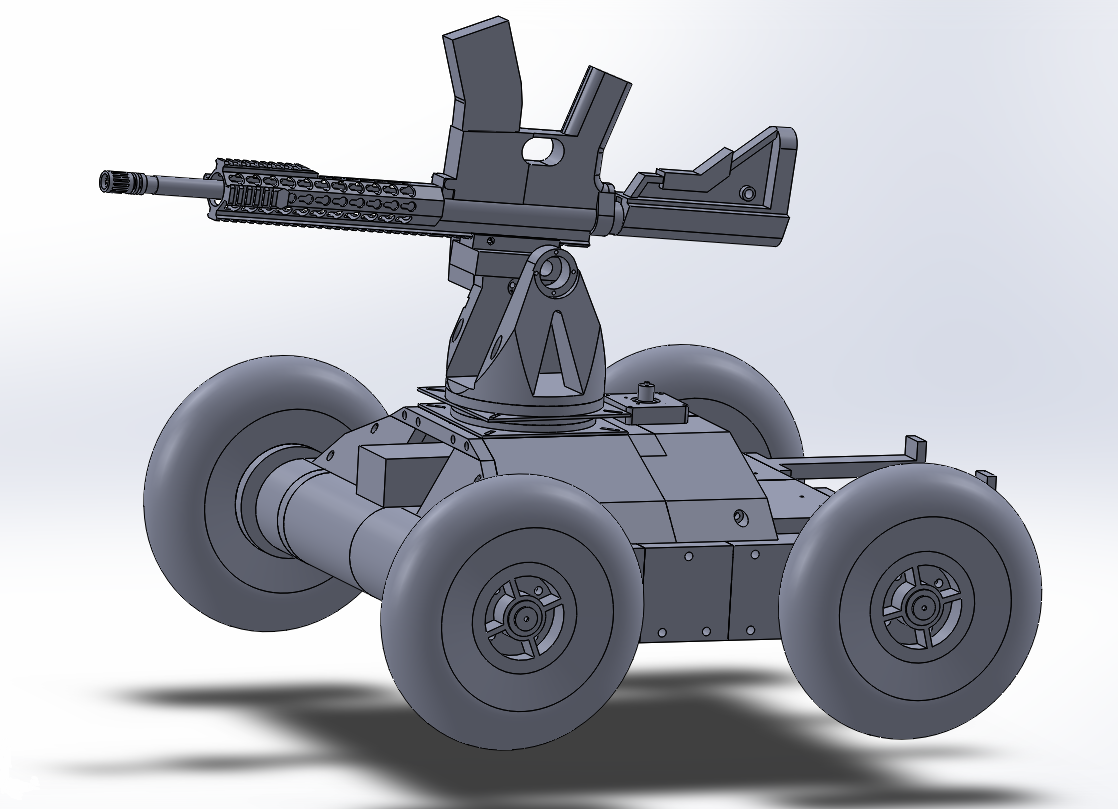
\includegraphics[width=1\textwidth]{Figures/robot_completo.png}
\label{fig:robot}
\caption{Robot completo}
\end{figure}

Para reducir tiempos y costos de prototipado se simularon por computadora las interacciones entre las piezas y la funcionalidad del prototipo lo que permitió que todas las partes funcionaran correctamente juntas antes de comenzar la impresión.

\subsection{Conclusiones del Análisis de Implementación}

El diseño del chasis se centro en los objetivos planteados para esta POC, se priorizo la facilidad de fabricación mediante impresión 3D y aseguro la modularidad y funcionalidad mecánica necesarias para el desplazamiento y operación del robot.

La estructura modular, segmentada en ejes, largueros, pisos, coraza y torreta, facilitó tanto el ensamblaje como la adaptación a cambios de diseño futuros.

Asimismo, se logró una integración estructural eficiente entre las piezas impresas, y un diseño que considera las limitaciones del volumen de impresión y maximiza la rigidez del conjunto. La simulación previa al prototipado físico permitió validar ensamblajes y detectar interferencias o problemas potenciales, y de esta manera reducir tiempos y costos en la fase de fabricación.